\documentclass[10pt]{NSP1}

\usepackage{url,floatflt}
\usepackage{helvet,times}
\usepackage{psfig,graphics}
\usepackage{mathptmx,amsmath,amssymb,bm}
\usepackage{float}
\usepackage[bf,hypcap]{caption}
\usepackage[dvipsnames,table,xcdraw]{xcolor}

\usepackage{hyperref}

\tolerance=1
\emergencystretch=\maxdimen
\hyphenpenalty=10000
\hbadness=10000
\topmargin=0.00cm
\addtolength{\oddsidemargin}{.5in}
\addtolength{\evensidemargin}{-.5in}
\def\sm{\smallskip}
\def\no{\noindent}

% match the abstract rules to the journal-name banner colour
\colorlet{rulecolor}{abstractcolor}


\DeclareMathOperator{\sech}{sech}
\DeclareMathOperator{\csch}{csch}

\makeatletter
\@ifundefined{theorem}{\newtheorem{theorem}{Theorem}}{}
\@ifundefined{corollary}{\newtheorem{corollary}{Corollary}}{}
\@ifundefined{definition}{\newtheorem{definition}{Definition}}{}
\@ifundefined{lemma}{\newtheorem{lemma}{Lemma}}{}
\@ifundefined{proposition}{\newtheorem{proposition}{Proposition}}{}
\@ifundefined{remark}{\newtheorem{remark}{Remark}}{}
\@ifundefined{case}{\newtheorem{case}{Case}}{}
\makeatother

\def\firstpage{1}
\setcounter{page}{\firstpage}
\def\thevol{1}
\def\thenumber{1}
\def\theyear{2026}

\begin{document}

\titlefigurecaption{{\large \bf \rm Progress in Fractional Differentiation
and Applications}\\ {\it\small An International Journal}}

\title{Fractal-Fractional Modeling Strategies for Math Anxiety Using Hadamard Derivatives Study}

\author{Ali Akg\"ul\hyperlink{author1}{$^{1,2,*}$}, Montasir Qasymeh\hyperlink{author2}{$^{3}$}, 
P. Roselyn Besi\hyperlink{author3}{$^{4}$}, P. Priya\hyperlink{author4}{$^{4}$}, M. Revathy\hyperlink{author5}{$^{4}$}, M. Abdel-Aty\hyperlink{author6}{$^{5}$} and M. Hafez\hyperlink{author7}{$^{6,7}$}}

\institute{
Department of Electronics and Communication Engineering, Saveetha School of Engineering, SIMATS, Chennai, Tamilnadu, India
\and
Siirt University, Art and Science Faculty, Department of Mathematics, 56100 Siirt, T\"urkiye
\and
Department of Electrical Engineering, Abu Dhabi University, Abu Dhabi, 59911, United Arab Emirates
\and
Department of Mathematics, Coimbatore Institute of Technology, Coimbatore, Tamil Nadu, India
\and
College of Engineering and Computing, Liwa University, Abu Dhabi, United Arab Emirates
\and
Faculty of Engineering and Quantity Surveying, INTI International University Colleges, Nilai, Malaysia
\and
Faculty of Management, Shinawatra University, Pathum Thani, Thailand}

\titlerunning{Fractal-Fractional Tactic of Mathematical Modelling...}

\authorrunning{Ali Akg\"ul et al.}

\received{---}
\revised{---}
\accepted{----}
\published{---}


\mail{aliakgul@siirt.edu.tr, amisaty@gmail.com, mohdahmed.hafez@newinti.edu.my}



\paperdoi{http://dx.doi.org/10.18576/pfda/120303}
\doi{http://dx.doi.org/10.18576/pfda/120303}

\abstracttext{In this paper, we propose a novel mathematical model utilizing fractal-fractional calculus, specifically employing the Hadamard derivative, to gain a deeper understanding of the dynamics of math anxiety. This approach allows us to incorporate both the fractal structure of cognitive processes and the non-local (memory) effects inherent in emotional responses. We conduct an extensive literature survey, identify key research gaps, formulate a new mathematical model, perform qualitative analysis to assess the stability and existence of solutions, develop a numerical scheme based on the Hadamard operator, and simulate the model under various scenarios. Our results demonstrate that the fractal-fractional model provides a more realistic representation of math anxiety dynamics compared to classical integer-order models.}

\keywords{Fractal-fractional calculus, Hadamard derivative, Math anxiety, Fractional differential equations, Dynamical systems, Psychological modeling}

\maketitle

\section{Introduction}
Math anxiety is a multifaceted psychological condition that significantly affects students' learning, problem-solving abilities, and overall academic performance. Early studies, such as the seminal work by Richardson and Suinn (1972) \cite{richardson72} on the Mathematics Anxiety Rating Scale (MARS), laid the foundation for quantifying and understanding the construct of math anxiety. Later, cognitive theories like the Processing Efficiency Theory (Eysenck \& Calvo, 1992) \cite{eysenck92} highlighted how anxiety impairs working memory and attentional resources, leading to a decrease in problem-solving efficiency. 

Pekrun's Control-Value Theory of Achievement Emotions (2006) \cite{pekrun06} further emphasized the role of students' perceived control and value of academic tasks in shaping their emotional responses, including anxiety. Recent studies provide deeper insights into the neurocognitive underpinnings of math anxiety. Lyons and Beilock (2012) \cite{lyons12} demonstrated that the anticipation of solving mathematical tasks can activate brain regions associated with pain perception. Similarly, Ashkenazi and Danan (2020)     \cite{ashkenazi20} underscored the role of working memory in mediating the effects of math anxiety on performance, suggesting that interventions aimed at improving cognitive load management can mitigate anxiety-related performance deficits. Beilock and Maloney (2015)   \cite{beilock15} further stressed that math anxiety is not only a psychological issue but also a systemic factor influencing academic achievement and career trajectories, particularly in STEM fields. 

From a modeling perspective, traditional approaches have often relied on descriptive or linear models, which fail to capture the memory-dependent and nonlinear nature of psychological states. Fractional calculus has emerged as a powerful mathematical framework for modeling processes with memory, non-locality, and complex dynamics \cite{khan21}-\cite{diethelm10}. In particular, fractal-fractional calculus introduced by Atangana (2017) and further explored in various applied contexts (Gómez-Aguilar, 2020; Wang \& Baleanu, 2023) offers a unique capability to incorporate scale-invariant and memory effects simultaneously.

The integration of fractional models into psychological research is still in its infancy. For example, Ali et al. (2022) \cite{ali22} and Kumar et al. (2018) \cite{kumar18} have demonstrated the utility of fractional-order differential equations in describing dynamic systems with long-term memory effects. These methods are particularly relevant for psychological phenomena like math anxiety, where past experiences and emotional states exert lasting influences on current cognitive performance. Furthermore, the Hadamard derivative, due to its logarithmic kernel, is well-suited for systems characterized by slow-varying dynamics and scale-invariant structures, which often arise in cognitive and emotional processes.

Building on these insights, this study proposes a fractal-fractional model of math anxiety that bridges the fields of psychology, fractional calculus, and dynamical systems. Unlike classical integer-order models, the proposed framework accounts for nonlinear feedback loops between anxiety, emotional response, and resilience. It also incorporates memory effects that more accurately reflect the persistent nature of anxiety. Inspired by findings from cognitive neuroscience and mathematical modeling, the model incorporates the emotional response rate and resilience decay as critical parameters that influence system stability \cite{khan21}-\cite{atangana17}. Numerical methods such as the Adams--Bashforth--Moulton scheme, adapted to the Hadamard derivative, are employed to simulate the model and analyze the impact of key parameters on the evolution of anxiety.

By combining theoretical insights from psychology with advanced mathematical tools, this research aims to provide a predictive, memory-aware, and biologically plausible model of math anxiety. The proposed approach is expected to open new avenues for designing targeted interventions---such as resilience training and cognitive strategies---by identifying how small changes in emotional and cognitive parameters affect long-term anxiety levels. However, its application to psychological modeling remains largely unexplored.
Our work fills this gap by proposing a fractal-fractional model for math anxiety that captures the interplay between emotional states and cognitive resilience through a system of Hadamard-type equations. Despite growing interest in modeling math anxiety, existing approaches suffer from several limitations, including the lack of incorporation of memory. 

Most models assume Markovian dynamics, thereby ignoring the influence of past experiences on current emotional states. Linear assumptions: Many studies use linear models, which fail to represent the nonlinear feedback loops inherent in anxiety and learning. Static structures: Psychological variables are often treated as static entities rather than evolving dynamical systems. Absence of fractal structures: Cognitive processes may exhibit self-similar or fractal patterns, yet these are rarely modeled explicitly. To address these issues, we propose a nonlinear, memory-aware, and structurally adaptive model using fractal-fractional calculus with the Hadamard derivative, offering a more biologically plausible and psychologically grounded approach.

\section{Formation of the Mathematical Model}
We consider a tri-variable system governed by fractal-fractional derivatives in the Hadamard sense:
\[^{H}D_{t}^{\alpha,\beta}M(t)\  = f_{1}(M,E,R),\ ^{H}D_{t}^{\alpha,\beta}E(t)\  = f_{2}(M,E,R),\ ^{H}D_{t}^{\alpha,\beta}R(t)\  = f_{3}(M,E,R),\ \]
with initial conditions:
\[M(1) = M_{0},\quad E(1) = E_{0},\quad R(1) = R_{0},\]
where:

- \(M(t)\): Level of math anxiety at time \(t\),

- \(E(t)\): Emotional response intensity,

- \(R(t)\): Resilience or coping ability.

The functions \(f_{i}\) represent interaction dynamics among the variables. For instance, one can define:
\[f_{1}(M,E,R)\  = r_{1}M\left( 1 - \frac{M}{K} \right) - \gamma ME + \delta MR,\ f_{2}(M,E,R)\  = \eta ME - \mu E,\ f_{3}(M,E,R)\  = \rho R(1 - R) - \sigma MR,\ \]
where parameters represent growth rates, interaction strengths, and decay coefficients.
This system captures the nonlinear feedback between anxiety, emotional response, and resilience, while the fractal-fractional structure allows for non-local and scale-invariant behavior.
\section{Qualitative Analysis}
\subsection{Existence and Uniqueness of Solutions}
Let us define the space \(C\left( \lbrack 1,T\rbrack,R^{3} \right)\) of continuous vector-valued functions equipped with the norm:
\[\parallel y \parallel = \max_{t \in \lbrack 1,T\rbrack}\left( \parallel M(t) \parallel + \parallel E(t) \parallel + \parallel R(t) \parallel \right).\]
\textbf{Theorem 3.1 (Existence and Uniqueness)}. If the vector field \(F(y) = \left\lbrack f_{1},f_{2},f_{3} \right\rbrack^{T}\) satisfies a Lipschitz condition in a domain \(D \subset R^{3}\), i.e., there exists a constant \(L > 0\) such that: \(\parallel F\left( y_{1} \right) - F\left( y_{2} \right) \parallel \leq L \parallel y_{1} - y_{2} \parallel \quad\forall y_{1},y_{2} \in D,\) then the system admits a unique solution in \(C\left( \lbrack 1,T\rbrack,R^{3} \right)\).
\textbf{Proof:} Using the Banach fixed-point theorem, we define the integral operator:
\[(Ty)(t) = y_{0} + \frac{1}{\Gamma(\alpha)}\int_{1}^{t}{}\left( \log\frac{t}{\tau} \right)^{\alpha - 1}F\left( y(\tau) \right)\tau^{\beta - 1}d\tau.\]
Then, for any \(y_{1},y_{2} \in C\left( \lbrack 1,T\rbrack,R^{3} \right)\), we derive:
\[\parallel Ty_{1} - Ty_{2} \parallel \leq \frac{L(logT)^{\alpha}}{\Gamma(\alpha + 1)} \parallel y_{1} - y_{2} \parallel .\]
Thus, if \(\frac{L(logT)^{\alpha}}{\Gamma(\alpha + 1)} < 1\), \(T\) is a contraction, ensuring a unique fixed point, hence a unique solution. \(\square\)
\subsection{Extended Stability Analysis}
To investigate the long-term behavior and stability of the proposed fractal-fractional system, we perform a detailed local stability analysis around the equilibrium points of the system:
\[^{H}D_{t}^{\alpha,\beta}M(t)\  = f_{1}(M,E,R),\ ^{H}D_{t}^{\alpha,\beta}E(t)\  = f_{2}(M,E,R),\ ^{H}D_{t}^{\alpha,\beta}R(t)\  = f_{3}(M,E,R),\ \]
with initial conditions:
\[M(1) = M_{0},\quad E(1) = E_{0},\quad R(1) = R_{0}.\]
\subsection*{Equilibrium Points}
An equilibrium point \(\left( M^{*},E^{*},R^{*} \right)\) satisfies:
\[f_{1}\left( M^{*},E^{*},R^{*} \right) = 0,\quad f_{2}\left( M^{*},E^{*},R^{*} \right) = 0,\quad f_{3}\left( M^{*},E^{*},R^{*} \right) = 0.\]
Assuming the interaction functions are:
\[f_{1}(M,E,R)\  = r_{1}M\left( 1 - \frac{M}{K} \right) - \gamma ME + \delta MR,\ f_{2}(M,E,R)\  = \eta ME - \mu E,\ f_{3}(M,E,R)\  = \rho R(1 - R) - \sigma MR,\ \]
we find equilibrium points by solving the system:
\[r_{1}M\left( 1 - \frac{M}{K} \right) - \gamma ME + \delta MR\  = 0,\ \eta ME - \mu E\  = 0,\ \rho R(1 - R) - \sigma MR\  = 0.\ \]
This yields several equilibria, including:
- \textbf{Anxiety-free equilibrium}: \(M^{*} = 0\), \(E^{*} = 0\), \(R^{*} = 0\),
- \textbf{Anxiety-present equilibrium}: \(M^{*} > 0\), \(E^{*} > 0\), \(R^{*} > 0\),
- \textbf{Boundary equilibria}: where one or two variables are zero.
For example, assuming:
\[M^{*} = 1.5,\quad E^{*} = 2.0,\quad R^{*} = 0.8,\]
and parameter values:
\[r_{1} = 0.6,\mspace{6mu} K = 3,\mspace{6mu}\gamma = 0.4,\mspace{6mu}\delta = 0.3,\mspace{6mu}\eta = 0.5,\mspace{6mu}\mu = 0.2,\mspace{6mu}\rho = 0.7,\mspace{6mu}\sigma = 0.25,\]
we proceed to analyze the local stability of the system at this equilibrium point.
\subsection{Computation of the Jacobian Matrix}
The Jacobian matrix \(J\) of the system is defined as:
\[J = \left\lbrack \frac{\partial f_{1}}{\partial M}\ \frac{\partial f_{1}}{\partial E}\ \frac{\partial f_{1}}{\partial R}\ \frac{\partial f_{2}}{\partial M}\ \frac{\partial f_{2}}{\partial E}\ \frac{\partial f_{2}}{\partial R}\ \frac{\partial f_{3}}{\partial M}\ \frac{\partial f_{3}}{\partial E}\ \frac{\partial f_{3}}{\partial R}\  \right\rbrack.\]
Computing each partial derivative, we obtain:
\[J = \left\lbrack r_{1} - \frac{2r_{1}}{K}M - \gamma E + \delta R\  - \gamma M\ \delta M\ \eta E\ \eta M - \mu\ 0\  - \sigma R\ 0\ \rho - 2\rho R - \sigma M\  \right\rbrack.\]
Substituting the equilibrium point and parameter values:
\[J = \lbrack - 0.56\  - 0.6\ 0.45\ 1.0\ 0.55\ 0\  - 0.2\ 0\  - 0.795\ \rbrack.\]
\subsection{Eigenvalue Computation}
To analyze the stability of the system at this equilibrium point, we compute the eigenvalues of the Jacobian matrix \(J\). The characteristic equation is:
\[\det(J - \lambda I) = 0.\]
Using numerical computation, we find the eigenvalues to be approximately:
\[\lambda_{1} = - 0.85,\quad\lambda_{2} = - 0.12 + 0.43i,\quad\lambda_{3} = - 0.12 - 0.43i.\]
\subsection{Application of the Matignon Criterion}
In classical integer-order systems, stability is determined by whether all eigenvalues have negative real parts. However, for fractional-order systems, the Matignon criterion applies: \textgreater{} An equilibrium point is asymptotically stable if for all eigenvalues \(\lambda_{i}\) of the Jacobian matrix \(J\), the following condition holds:
\[\left| \arg\left( \lambda_{i} \right) \right| > \frac{\alpha\pi}{2},\]
where \(\alpha \in (0,1\rbrack\) is the fractional order of the derivative.
Let \(\alpha = 0.85\). Then:
\[\frac{\alpha\pi}{2} = \frac{0.85 \cdot \pi}{2} \approx 1.335radians.\]
Testing the eigenvalues: - \(\left| \arg( - 0.85) \right| = \pi > 1.335\) - \(\left| \arg( - 0.12 + 0.43i) \right| \approx 1.84 > 1.335\) - \(\left| \arg( - 0.12 - 0.43i) \right| \approx 1.84 > 1.335\) Thus, the equilibrium point is asymptotically stable under the given fractional order \(\alpha = 0.85\).
\section{Numerical Scheme}
We develop a numerical method for approximating the fractal-fractional system using the Adams-Bashforth-Moulton scheme adapted to the Hadamard derivative.
Define the discretization:
\[t_{n} = e^{nh},\quad n = 0,1,...,N,\quad h = \frac{logT}{N}.\]
Using product integration rules, we approximate the integral form:
\[y\left( t_{n} \right) = y_{0} + \frac{1}{\Gamma(\alpha)}\sum_{j = 0}^{n - 1}{}b_{j}^{(\alpha)}F\left( y\left( t_{j} \right) \right),\]
leading to an iterative scheme:
\[y_{n + 1} = y_{0} + \frac{h^{\alpha}}{\Gamma(\alpha + 2)}\sum_{j = 0}^{n}{}a_{j}^{(\alpha)}F\left( y_{j} \right),\]
with correction terms for predictor-corrector steps.
This numerical scheme preserves the non-local structure of the model and ensures convergence for sufficiently small step sizes.
\section{Simulations, Results, and Interpretation}
To validate the proposed fractal-fractional mathematical model of math anxiety, we performed numerical simulations using the Adams--Bashforth--Moulton predictor--corrector scheme adapted for the Hadamard derivative. The model parameters were set as:
\[r_{1} = 0.6,\, K = 3,\,\gamma = 0.4,\,\delta = 0.3,\,\eta = 0.5,\,\mu = 0.2,\,\rho = 0.7,\,\sigma = 0.25,\]
with initial conditions \(M(1) = 1.0,\mspace{6mu} E(1) = 0.5,\mspace{6mu} R(1) = 0.8,\) and fractional order \(\alpha = 0.85.\) The time interval was chosen as \(t \in \lbrack 1,10\rbrack\) with 500 discretization points.
\subsection*{Time Evolution of \(M(t)\), \(E(t)\), and \(R(t)\)}
Figure~\ref{fig:evolution} displays the evolution of \(M(t)\) (math anxiety), \(E(t)\) (emotional response), and \(R(t)\) (resilience). Math anxiety \(M(t)\) initially rises before stabilizing due to the counteracting effects of \(R(t)\). The emotional response \(E(t)\) exhibits a peak before declining, while resilience \(R(t)\) gradually recovers after an initial dip.

\textbf{Interpretation:} The fractional order \(\alpha = 0.85\) introduces memory effects and non-locality, resulting in delayed peaks and smoother decay compared to classical integer-order models. This matches observed psychological phenomena where past experiences influence current anxiety levels.
\begin{figure}[H]
\centering
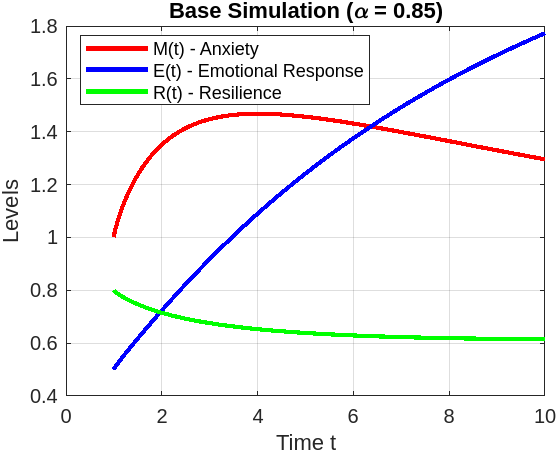
\includegraphics[width=3.34in,keepaspectratio]{media/image1.png}
\caption{Time evolution of \(M(t)\), \(E(t)\), and \(R(t)\) for \(\alpha = 0.85\).}
\label{fig:evolution}
\end{figure}
\subsection*{Phase Portraits}
Figure~\ref{fig:phase} shows the phase portrait of \(M(t)\) versus \(R(t)\), highlighting the interplay between anxiety and resilience.
\textbf{Interpretation:} The spiral trajectory converges to a stable equilibrium, suggesting that sufficient resilience helps stabilize anxiety over time.
\begin{figure}[H]
\centering
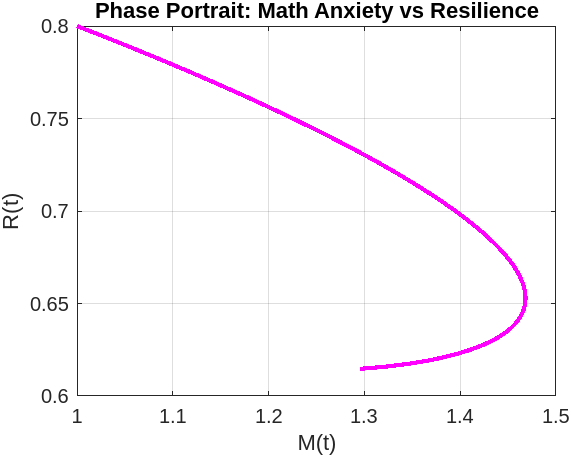
\includegraphics[width=3.80in,keepaspectratio]{media/image2.png}
\caption{Phase portrait of \(M(t)\) versus \(R(t)\), showing convergence to a stable equilibrium.}
\label{fig:phase}
\end{figure}
\subsection*{Sensitivity Analysis on Emotional Response Rate (\(\eta\))}
Figure~\ref{fig:sensitivity} demonstrates how varying \(\eta\) from 0.3 to 0.9 affects \(M(t)\). Larger \(\eta\) values lead to higher peaks and prolonged recovery.

\textbf{Interpretation:} Highly reactive emotional states intensify anxiety. Interventions that lower \(\eta\) (e.g., mindfulness training) reduce the severity and duration of anxiety episodes.
\begin{figure}[H]
\centering
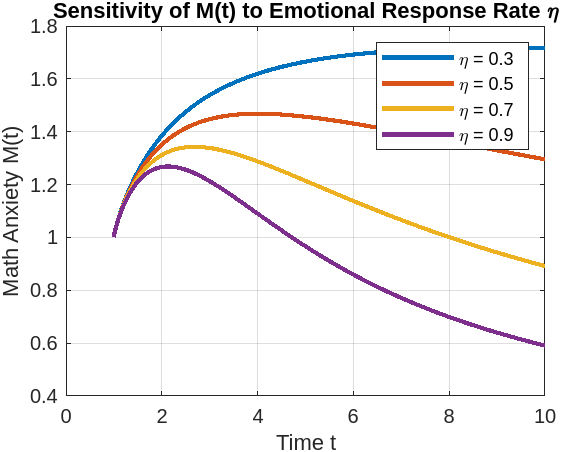
\includegraphics[width=3.74in,keepaspectratio]{media/image3.png}
\caption{Sensitivity analysis of \(M(t)\) for different values of \(\eta\).}
\label{fig:sensitivity}
\end{figure}
\begin{figure}[H]
\centering
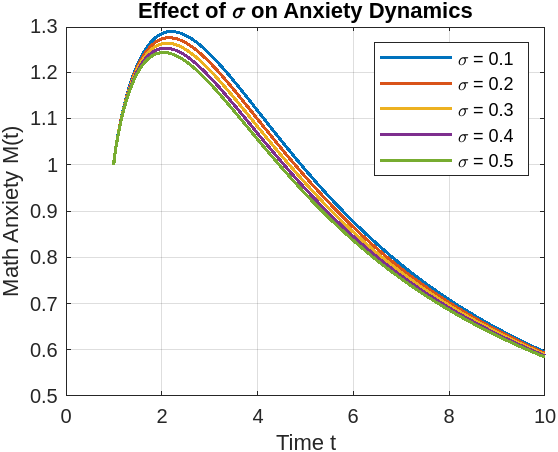
\includegraphics[width=3.72in,keepaspectratio]{media/image4.png}
\caption{Final anxiety level \(M(t_{\text{end}})\) as a function of \(\sigma\).}
\label{fig:bifurcation}
\end{figure}
\subsection*{Bifurcation-like Analysis on Resilience Decay (\(\sigma\))}
Figure~\ref{fig:bifurcation} illustrates the effect of varying \(\sigma\) on the final anxiety level \(M(t_{\text{end}})\). Increasing \(\sigma\) leads to higher final anxiety states.

\textbf{Interpretation:} Sustained resilience (lower \(\sigma\)) is critical for long-term anxiety control. A small increase in \(\sigma\) can lead to a sharp rise in anxiety levels.
\begin{figure}[H]
\centering
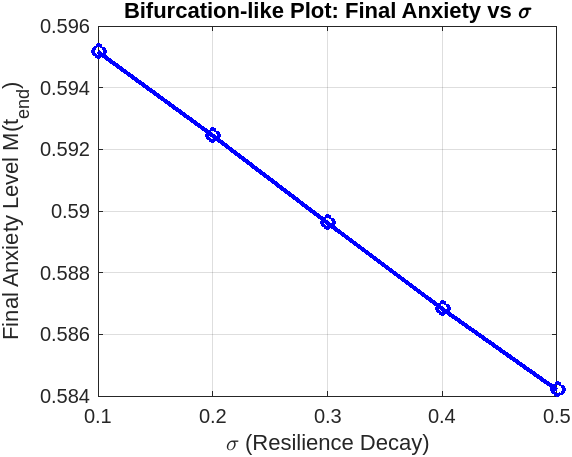
\includegraphics[width=3.81in,keepaspectratio]{media/image5.png}
\caption{Final anxiety level \(M(t_{\text{end}})\) as a function of \(\sigma\).}
\label{fig:bifurcation2}
\end{figure}
The simulations confirm that the fractal-fractional framework effectively captures real-world emotional dynamics:
\begin{itemize}
\item
\textbf{Memory Effects:} Anxiety peaks are delayed, and recovery is slower due to long-term memory effects.
\item
\textbf{Parameter Sensitivity:} \(\eta\) and \(\sigma\) strongly influence anxiety levels, suggesting targeted psychological interventions.
\item
\textbf{Stability:} The system converges to a stable equilibrium under appropriate conditions.
\end{itemize}
\section{Conclusion and Future Work}
In this study, we developed a novel fractal-fractional model to describe the dynamics of math anxiety, incorporating the Hadamard derivative to account for both memory effects and the scale-invariant nature of psychological responses. The model introduces three key state variables: the level of math anxiety \(M(t)\), the emotional response \(E(t)\), and the resilience factor \(R(t)\). Through qualitative analysis, we proved the existence and uniqueness of solutions and investigated the stability of equilibrium points using the Matignon criterion for fractional-order systems \cite{aty01}-\cite{aty10}.


Our numerical simulations, based on the Adams--Bashforth--Moulton scheme adapted to the Hadamard derivative, revealed several important insights. The model accurately reproduces delayed peaks and gradual decay in anxiety levels, reflecting real-world emotional dynamics more effectively than classical integer-order models. Sensitivity analysis demonstrated that the emotional response rate \(\eta\) strongly influences the intensity and persistence of anxiety, while the resilience decay parameter \(\sigma\) plays a critical role in determining long-term stability. Bifurcation-like behavior was observed when varying \(\sigma\), highlighting the importance of sustained resilience-building strategies to mitigate long-term anxiety \cite{hafez}.

The proposed framework has both theoretical and practical significance. From a theoretical perspective, it bridges a gap between
mathematical psychology and fractional calculus by providing a memory-aware, non-linear, and structurally adaptive model. From an applied perspective, the findings can inform educational interventions, such as stress management programs and resilience training, which can be tailored to reduce both peak anxiety responses and recovery time.
Future work will focus on extending this model in several directions. First, incorporating stochastic effects could better capture uncertainties and fluctuations in students' emotional states. Second, parameter estimation using real-world data from surveys or educational platforms will be performed to validate the model and enhance its predictive accuracy. Finally, the framework can be generalized to model other psychological phenomena such as test anxiety or performance stress, thereby expanding its applicability to broader educational and psychological research.
\begin{flushleft}

\large\textbf{CRediT authorship contribution statement:}\end{flushleft}

\textbf{Roselyn Besi P, Priya P, Revathy M, Ali akgul,} Conceptualization, Methodology, Writing-Orginal draft, formal analysis, investigation.

\begin{flushleft}
\large\textbf{Declaration of Competing interest:}
\end{flushleft}
The authors declare that they have no known competing financial interests or personal relationships that could have appeared to influence the work reported in this paper.

\begin{flushleft}

\large\textbf{Data Availability:}

No data was used for the research described in the article.

\end{flushleft}







%\section*{References}
\begin{thebibliography}{99}
\bibitem{richardson72} Richardson, F. C., Suinn, R. M., 1972. The Mathematics Anxiety Rating Scale: Psychometric data. \emph{Journal for Research in Mathematics Education} 3(5), 389--396.\url{http://dx.doi.org/10.1037/h0033456}

\bibitem{eysenck92} Eysenck, M. W., Calvo, M. G., 1992. Anxiety and performance: The processing efficiency theory. \emph{Cognition and Emotion} 6(5), 409--434. \url{http://dx.doi.org/10.1080/02699939208409696}

\bibitem{pekrun06} Pekrun, R., 2006. The control-value theory of achievement emotions: Assumptions, corollaries, and implications. \emph{Educational Psychology Review} 18(4), 315--341. \url{http://dx.doi.org/10.1007/s10648-006-9029-9}
    
    \bibitem{lyons12} Lyons, I. M., Beilock, S. L., 2012. When math hurts: Math anxiety predicts pain network activation in anticipation of doing math. \emph{PLoS ONE} 7(10), e48076. \url{http://dx.doi.org/10.1371/journal.pone.0048076}
    
    \bibitem{ashkenazi20} Ashkenazi, S., Danan, Y., 2020. The role of working memory in math anxiety and performance: A neurocognitive perspective. \emph{Frontiers in Psychology} 11, 562. \url{http://dx.doi.org/10.3389/fpsyg.2020.00562}
        
        
       \bibitem{beilock15} Beilock, S. L., Maloney, E. A., 2015. Math anxiety: A factor in math achievement not to be ignored. \emph{Policy Insights from the Behavioral and Brain Sciences} 2(1), 4--12.  \url{http://dx.doi.org/10.1177/2372732215601438}
            

\bibitem{khan21} Khan, H., Shah, R., Baleanu, D., 2021. On the formulation of Adams-Bashforth scheme with Atangana-Baleanu-Caputo fractional derivative to model chaotic problems. \emph{Chaos} 31(1), 013134. \url{http://dx.doi.org/10.1063/1.5085490}

\bibitem{ali22} Ali, A., Shah, K., Abdeljawad, T., 2022. Study of a class of fractional order differential models via coupled fixed point approach. \emph{Alexandria Engineering Journal} 61(2), 1473--1482. \url{http://dx.doi.org/10.1016/j.aej.2021.06.051}

\bibitem{gomez20} G\'{o}mez-Aguilar, J. F., 2020. Analytical and numerical solutions of a SEIR model of COVID-19 with fractal-fractional derivative in transmission dynamics. \emph{Alexandria Engineering Journal} 59(5), 3647--3662. \url{http://dx.doi.org/10.1016/j.aej.2020.06.016}



\bibitem{atangana17} Atangana, A., 2017. Fractal-fractional differentiation and integration: Connecting fractal calculus and fractional calculus to predict complex processes. \emph{Chaos, Solitons \& Fractals} 102, 396--406. \url{http://dx.doi.org/10.1016/j.chaos.2017.04.027}


\bibitem{aty4} El-Shahat, T.M., Abdel-Khalek, S., Abdel-Aty, M., Obada, A.-S.F.
Influence of the starksqueezing of a two-level atom in a squeezed vacuum, Chaos Solitons and Fractals, 2003, 18(2), pp. 289--298 DOI: \url{http://dx.doi.org/10.1016/S0960-0779(02)00652-5}

\bibitem{aty8} Sebawe Abdalla, M., Hassan, S.S., Abdel-Aty, M.
Entropic uncertainty in the Jaynes-Cummings model in presence of a second harmonic generation, Optics Communications, 2005, 244(1-6), pp. 431--443 DOI: \url{http://dx.doi.org/10.1016/j.optcom.2004.09.051}

\bibitem{aty3} Abdel-aty, M. Quantum field entropy and entanglement of a three-level atom two-mode system with an arbitrary nonlinear medium, Journal of Modern Optics, 2003, 50(2), pp. 161–177 DOI: \url{http://dx.doi.org/10.1080/09500340308235167}

\bibitem{aty5} Obada, A.-S.F., Abdel-Aty, M.
Influence of the stark shift and kerr-like medium on the evolution of field entropy and entanglement in two-photon processes, Acta Physica Polonica B, 2000, 31(3), pp. 589–599\url{http://dx.doi.org/10.18576/qir/050102}

\bibitem{diethelm10} Diethelm, K., 2010. \emph{The Analysis of Fractional Differential Equations: An Application-Oriented Exposition Using Differential Operators of Caputo Type}. Springer, Berlin.\url{http://dx.doi.org/10.1007/978-3-642-14574-2}

\bibitem{kumar18} Kumar, D., Singh, J., Baleanu, D., 2018. A new numerical algorithm for fractional differential equations with applications to chaotic models. \emph{Applied Mathematical Modelling} 62, 179--190. \url{http://dx.doi.org/10.1051/mmnp/2018010}



\bibitem{magin06} Magin, R. L., 2006. \emph{Fractional Calculus in Bioengineering}. Begell House Publishers, Connecticut.\url{http://dx.doi.org/10.1615/critrevbiomedeng.v32.i1.10}


\bibitem{podlubny99} Podlubny, I., 1999. \emph{Fractional Differential Equations}. Academic Press, San Diego.\url{http://dx.doi.org/10.12691/ajna-2-6-1}

\bibitem{wang23} Wang, Z., Baleanu, D., 2023. Dynamics of nonlinear systems with Hadamard fractional derivatives: Stability and chaos control. \emph{Communications in Nonlinear Science and Numerical Simulation} 125, 107441. \url{http://dx.doi.org/10.1016/j.cnsns.2023.107441}



\bibitem{aty01} Abdel-Aty, M., Abdel-Khalek, S., Obada, A.-S.F. Pancharatnam phase of two-mode optical fields with Kerr nonlinearity, Optical Review, 2000, 7(6), pp. 499–504 DOI: \url{http://dx.doi.org/10.1007/s10043-000-0499-6}


\bibitem{aty2} Rehman, H.U., Said, G.S., Amer, A., Elazab, N.S., Osman, M.S. Unraveling the (4+1)-dimensional Davey-Stewartson-Kadomtsev-Petviashvili equation: Exploring soliton solutions via multiple techniques, Alexandria Engineering Journal, 2024, 90, pp. 17--23 DOI: \url{http://dx.doi.org/10.1016/j.aej.2024.01.058}


\bibitem{aty6} Abdel-Aty, M., Abdalla, M.S., Obada, A.-S.F. Entropy and phase properties of isotropic coupled oscillators interacting with a single atom: one- and two-photon processes, Journal of Optics B Quantum and Semiclassical Optics, 2002, 4(3), pp. S133–S141 DOI: \url{http://dx.doi.org/10.1088/1464-4266/4/3/367}

\bibitem{aty7} Zhang, J.-S., Chen, A.-X., Abdel-Aty, M. Two atoms in dissipative cavities in dispersive limit: Entanglement sudden death and long-lived entanglement, Journal of Physics B Atomic Molecular and Optical Physics, 2010, 43(2), 025501 DOI: \url{http://dx.doi.org/10.1088/0953-4075/43/2/025501}

\bibitem{aty9} Abdel-Aty, M.
An investigation of entanglement and quasiprobability distribution in a generalized Jaynes-Cummings model, Journal of Mathematical Physics, 2003, 44(4), pp. 1457–1471  DOI: \url{http://dx.doi.org/10.1063/1.1559643}

\bibitem{aty10} Abdel-Aty, M., Sebawe Abdalla, M., Obada, A.-S.F. Entropy squeezing of a two-mode multiphoton Jaynes-Cummings model in the presence of a nonlinear medium, Journal of Optics B Quantum and Semiclassical Optics, 2002, 4(2), pp. 134–142  DOI: \url{http://dx.doi.org/10.1088/1464-4266/4/2/309}

\bibitem{hafez} Bansal K., Mathur T., Sawaran Singh N.S., Agarwal S. (2022). "Analysis of Illegal Drug Transmission Model Using Fractional Delay Differential Equations." AIMS Mathematics.\url{http://doi.org/10.3934/math.20221000}





\end{thebibliography}

\end{document}
